\documentclass[tikz,border=15pt]{standalone}
\usepackage{sansmath}
\usepackage{siunitx}
\usetikzlibrary{decorations.text}

\usepackage[T1]{fontenc}					%Schriften unterschiedlicher Kodierung
\usepackage[utf8]{inputenc}	

\begin{document}
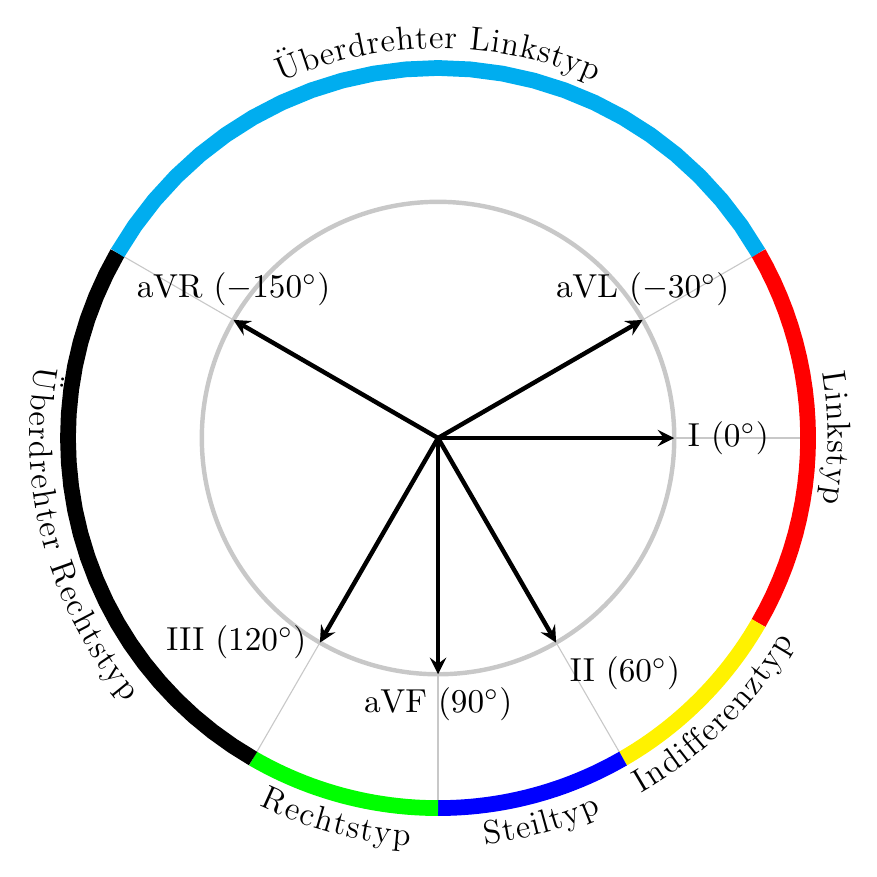
\begin{tikzpicture}

\def\size{3}
\def\textsize{1.2}
\definecolor{brightgray}{RGB}{200,200,200}
\definecolor{brightblue}{RGB}{150,150,255}
\def\outersize{4.7}
\def\outerfontsize{13}

\coordinate (center) at (0, 0);

\draw[ultra thick, brightgray] (center) circle (\size cm);

% Typentrennlinien
\draw[brightgray] ({\size*cos(0)}, {-\size*sin(0)}) -- ({\outersize*cos(0)}, {-\outersize*sin(0)});

\draw[brightgray] ({\size*cos(60)}, {-\size*sin(60)}) -- ({\outersize*cos(60)}, {-\outersize*sin(60)});

\draw[brightgray] ({\size*cos(90)}, {-\size*sin(90)}) -- ({\outersize*cos(90)}, {-\outersize*sin(90)});

\draw[brightgray] ({\size*cos(120)}, {-\size*sin(120)}) -- ({\outersize*cos(120)}, {-\outersize*sin(120)});

\draw[brightgray] ({\size*cos(-150)}, {-\size*sin(-150)}) -- ({\outersize*cos(-150)}, {-\outersize*sin(-150)});

\draw[brightgray] ({\size*cos(-30)}, {-\size*sin(-30)}) -- ({\outersize*cos(-30)}, {-\outersize*sin(-30)});

% Ableitungspfeile
\draw[ultra thick, ->, >=stealth] (center) --  ({\size*cos(0)}, {\size*sin(0)}) node[right, scale=\textsize] {I ($\ang{0}$)};

\draw[ultra thick, ->, >=stealth] (center) -- ({\size*cos(60)}, {-\size*sin(60)}) node[below right, scale=\textsize] {II ($\ang{60}$)};

\draw[ultra thick, ->, >=stealth] (center) -- ({\size*cos(120)}, {-\size*sin(120)}) node[left, scale=\textsize] {III ($\ang{120}$)};

\draw[ultra thick, ->, >=stealth] (center) -- ({\size*cos(90)}, {-\size*sin(90)}) node[below, scale=\textsize] {aVF ($\ang{90}$)};

\draw[ultra thick, ->, >=stealth] (center) -- ({\size*cos(-30)}, {-\size*sin(-30)}) node[above, scale=\textsize] {aVL ($\ang{-30}$)};

\draw[ultra thick, ->, >=stealth] (center) -- ({\size*cos(-150)}, {-\size*sin(-150)}) node[above, scale=\textsize] {aVR ($\ang{-150}$)};


% Typenfarben
\draw [red,line width=2mm,domain=-30:30] plot ({\outersize*cos(-\x)}, {\outersize*sin(-\x)});
\draw [yellow,line width=2mm,domain=30:60] plot ({\outersize*cos(-\x)}, {\outersize*sin(-\x)});
\draw [blue,line width=2mm,domain=60:90] plot ({\outersize*cos(-\x)}, {\outersize*sin(-\x)});
\draw [green,line width=2mm,domain=90:120] plot ({\outersize*cos(-\x)}, {\outersize*sin(-\x)});
\draw [black,line width=2mm,domain=120:210] plot ({\outersize*cos(-\x)}, {\outersize*sin(-\x)});
\draw [cyan,line width=2mm,domain=-30:-150] plot ({\outersize*cos(-\x)}, {\outersize*sin(-\x)});

% Tyoenbeschriftungen
\draw[draw=none, rotate=180, postaction={decorate, decoration={text along path, text format delimiters={|}{|}, raise=7pt, text align={align=center}, text={|\fontsize{\outerfontsize}{0}\selectfont|Linkstyp}, reverse path}}] (0,0) circle (\outersize);

\draw[draw=none, rotate=135, postaction={decorate, decoration={text along path, text format delimiters={|}{|}, raise=-14pt, text align={align=center}, text={|\fontsize{\outerfontsize}{0}\selectfont|Indifferenztyp}}}] (0,0) circle (\outersize);

\draw[draw=none, rotate=105, postaction={decorate, decoration={text along path, text format delimiters={|}{|}, raise=-14pt, text align={align=center}, text={|\fontsize{\outerfontsize}{0}\selectfont|Steiltyp}}}] (0,0) circle (\outersize);

\draw[draw=none, rotate=75, postaction={decorate, decoration={text along path, text format delimiters={|}{|}, raise=-14pt, text align={align=center}, text={|\fontsize{\outerfontsize}{0}\selectfont|Rechtstyp}}}] (0,0) circle (\outersize);

\draw[draw=none, rotate=15, postaction={decorate, decoration={text along path, text format delimiters={|}{|}, raise=-14pt, text align={align=center}, text={|\fontsize{\outerfontsize}{0}\selectfont|{Ü}berdrehter Rechtstyp}}}] (0,0) circle (\outersize);

\draw[draw=none, rotate=-90, postaction={decorate, decoration={text along path, text format delimiters={|}{|}, raise=7pt, text align={align=center}, text={|\fontsize{\outerfontsize}{0}\selectfont|{Ü}berdrehter Linkstyp}, reverse path}}] (0,0) circle (\outersize);

\end{tikzpicture}


\end{document}